% Activate the following line by filling in the right side. If for example the name of the root file is Main.tex, write
% "...root = Main.tex" if the chapter file is in the same directory, and "...root = ../Main.tex" if the chapter is in a subdirectory.
 
%!TEX root =  ../plantillaTFG.tex 
%recuerda que si cambias el nombre del fichero... debes cambiarlo aqui
\chapter{Data Preparation}
The main objective of our project is to identify risk zones where potential contact between power lines and vegetation could occur in the region of Cantabria. Thus, satellite imagery data related to vegetation (or more broadly, landcover) is required, along with corresponding masks that outline vegetation areas for model training (preferably specific to Cantabria, if available). In addition to vegetation data, geospatial data on the location of power lines is also needed for analyzing intersection zones. 
\newpage
\section{Copernicus data}
\begin{figure}[H]
 \centering
 \includegraphics[scale=0.8]{IMAGENES/IMG10-sentinel2.png}
 \captionsetup{font=large}
 \caption {Sentinel 2A imagery, with only RGB channels.}
\end{figure}

For the vegetation dataset, our initial approach was to create a custom dataset. We began by exploring open-access imagery from Sentinel-2 mission. To load and visualize this data, we utilized the Copernicus API with an open-source GIS application called QGIS. The imagery obtained is composed of multiple spectrums in different
spatial resolutions (for example, in visible bands, the resolution is 10 m/pixel), these bands could be used to determine some important indices, such as the Normalized Difference Vegetation Index (NDVI), which is useful for identifying vegetation. However, during the data processing phase, we have encountered 2 problems:\\

\begin{itemize}
    \item \textbf{Complexity in manaing spectrums}: As previously mentioned, the images are composed of multiple spectrums (not just the standard RGB channels), and this presents a problem for model training, because we need to decide whether to include all available spectral bands (Sentinel-2 satellite images include a total of 13 spectral bands) or restrict the input to only the RGB channels. This decision must be made at the beginning, as once a model is trained, its architecture and weights are fixed. Consequently, the model can only perform inference on images with the same number and type of channels used during training. In other words, if the model was trained on all 13 spectral bands, it cannot perform inference on input image that has only RGB bands.\\ 
    \item \textbf{Manual annotation}: These data lack corresponding segmentation masks, meaning that any further processing would require creating them from scratch through manual annotation, which is highly time-consuming and labor-intensive.
    


\end{itemize}
Given the limited timeframe for project implementation, we considered that relying on the initially planned data sources was not feasible. Consequently, an alternative approach was explored, focusing on more suitable sources of satellite imagery that already included pre-annotated masks.
\section{Jordan Forest Dataset (Training set):}
\begin{figure}[H]
\centering
\begin{subfigure}{0.49\textwidth}
\centering
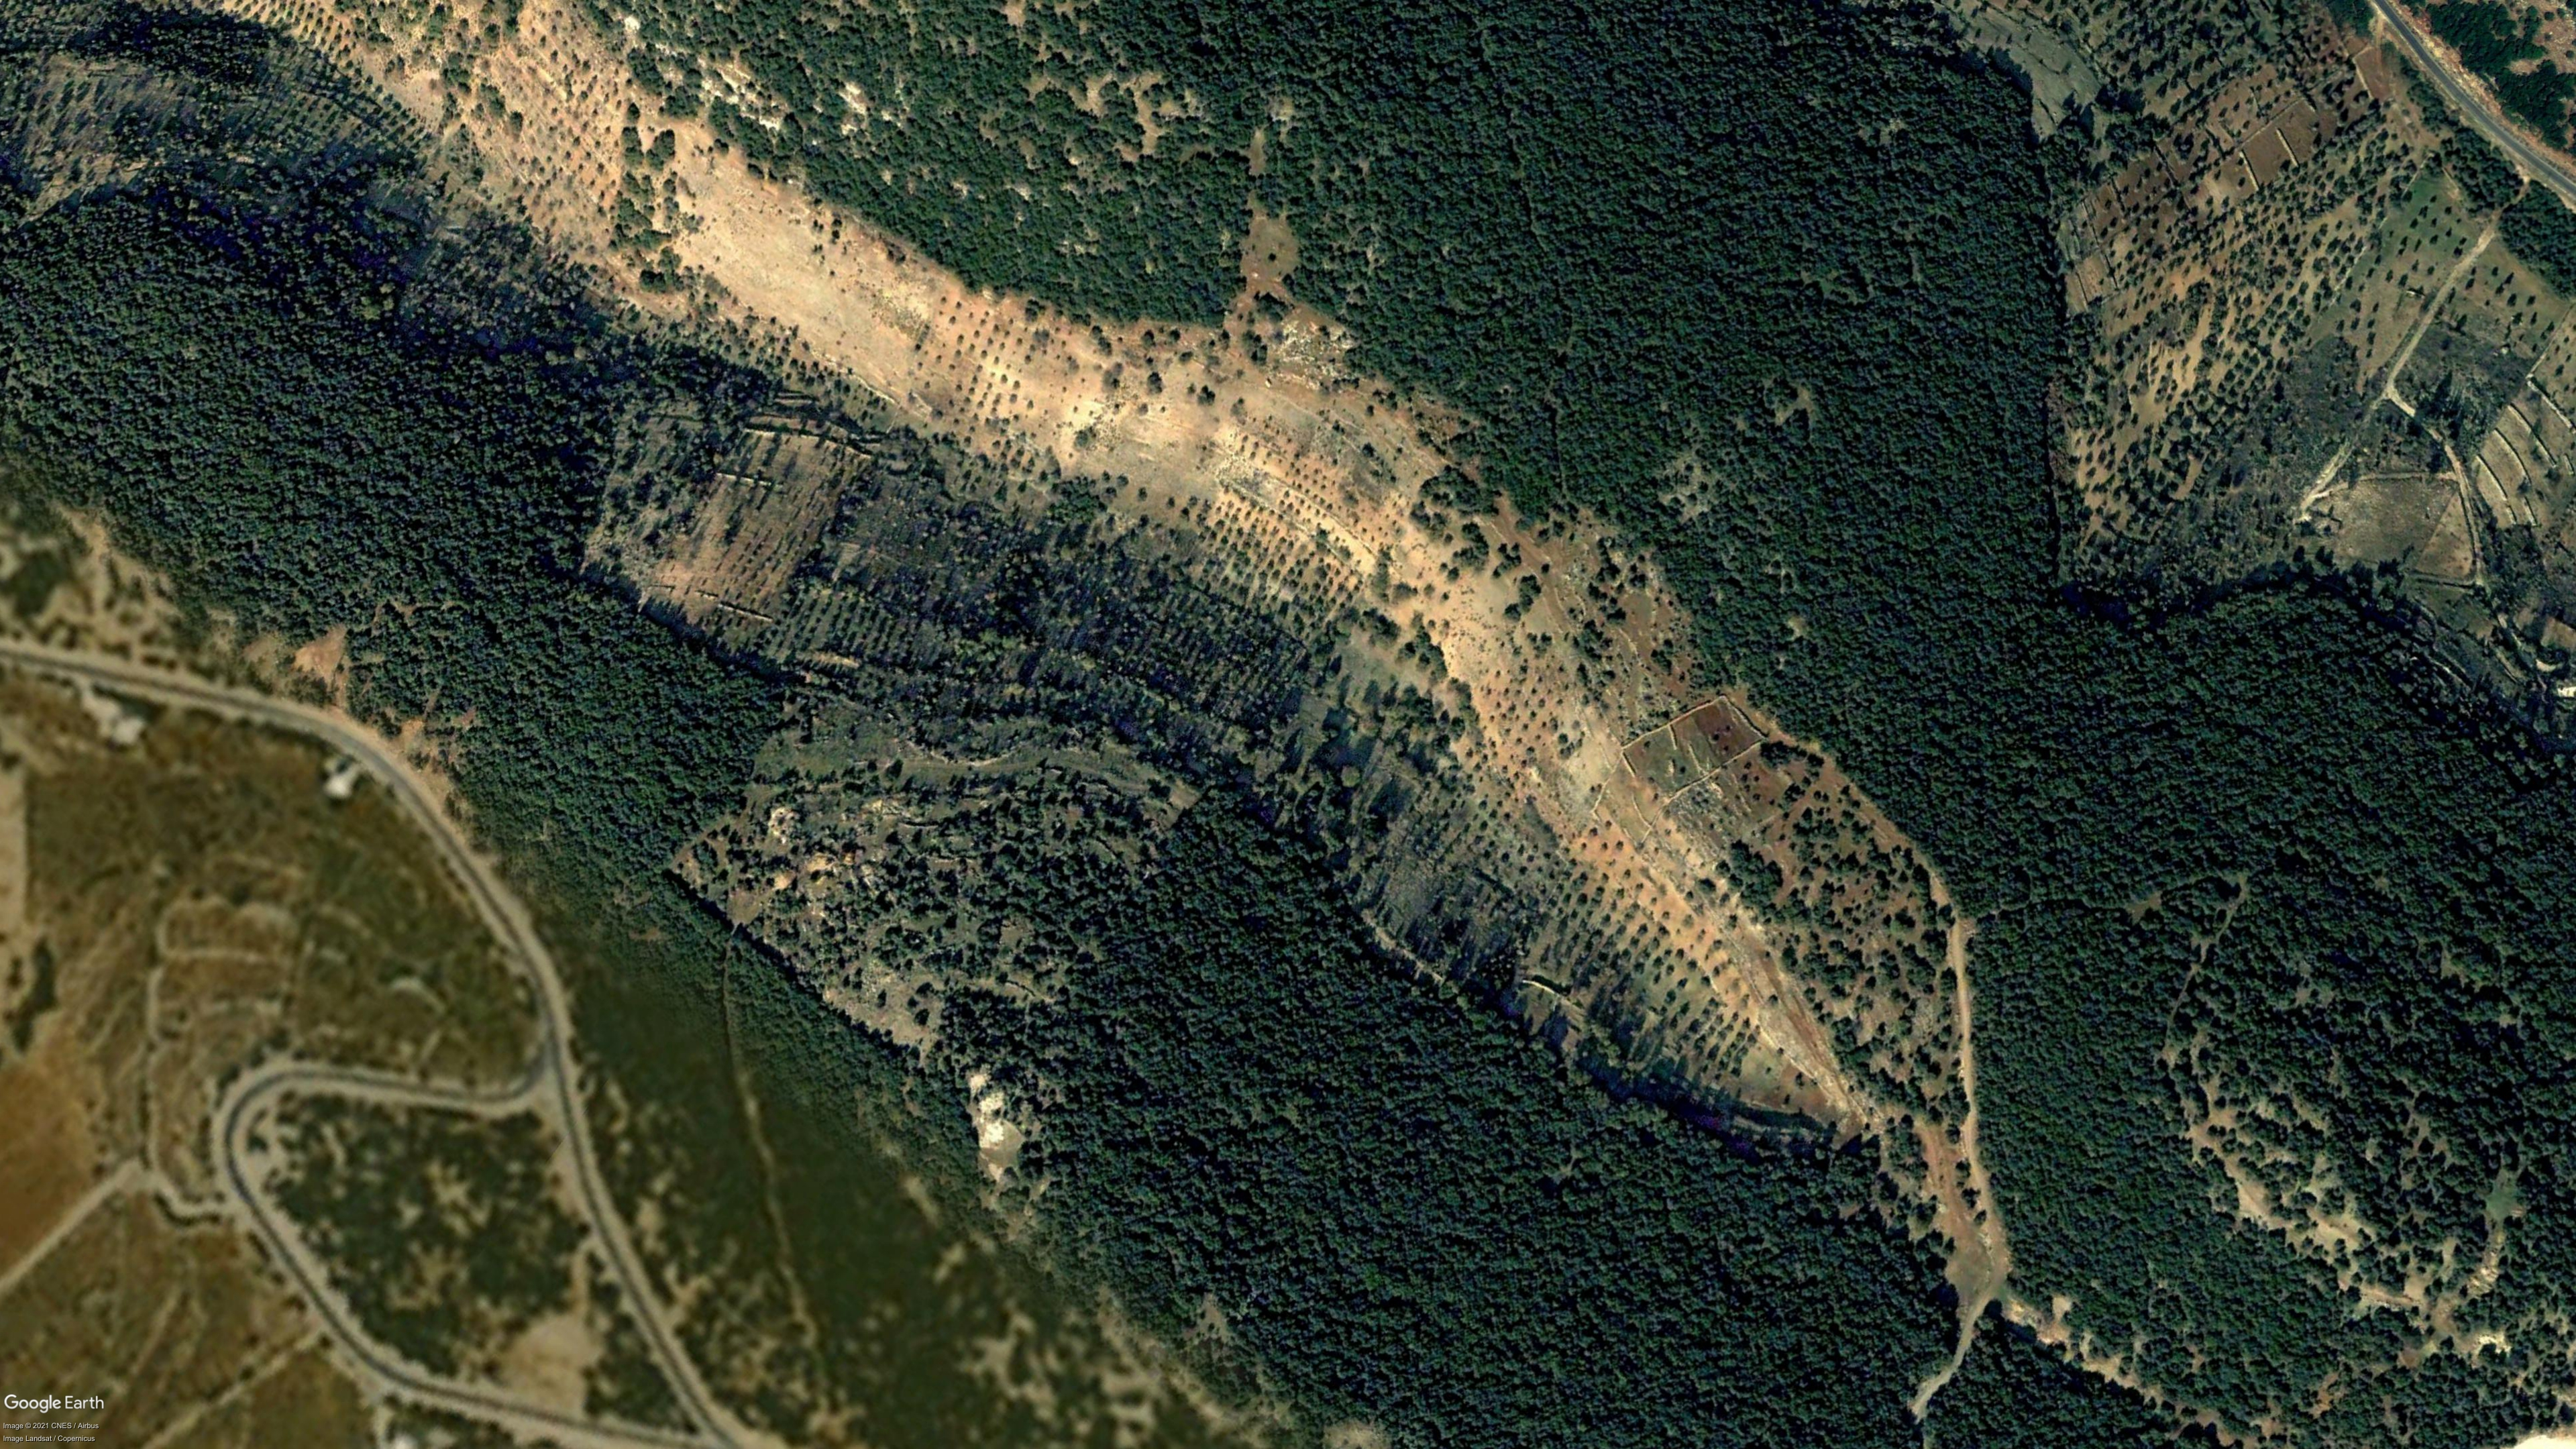
\includegraphics[width = \textwidth]{IMAGENES/IMG11-IMG.jpg}
\caption{Jordan Forest Dataset (Image)}
\label{fig:left}
\end{subfigure}
\begin{subfigure}{0.49\textwidth}
\centering
\includegraphics[width = \textwidth]{IMAGENES/IMG11-MASK.png}
\caption{Jordan Forest Dataset  (Mask)}
\label{fig:right}
\end{subfigure}
\caption{Jordan Forest Dataset (Images extracted from[21])}
\label{fig:combined}
\end{figure}


\textbf{Description}: 
\\
The Jordan Forests Dataset was obtained from a data science community called Kaggle [18]. It contains a collection of 4,576 cloud-free Landsat-8 satellite images, each with a spatial dimension of 2160 x 3840 pixels (30 m/pixel). Despite the images have a lower resolution comparing with those of Sentinel-2 (10 m/pixel for visible bands), the dataset includes both the original RGB satellite images and the corresponding ground-truth forest masks, therefore no manual annotation is required. The imagery spans a ten-year period from 2010 to 2020, covering five major forested regions in Jordan.\\ 

\textbf{Curation}: 
\\
In the ground-truth masks, the forest regions are highlighted in green, while the remaining non-forest areas are considered as background and marked white (these masks are provided in RGB format rather than binary). As part of the preprocessing pipeline, we have converted the masks into binary format, assigning a value of 1 to forested pixels and 0 to the background (non-forest areas).\\

\section{Loveda dataset (Training set):}
 \begin{figure}[H]
\centering
\begin{subfigure}{0.49\textwidth}
\centering
\includegraphics[width = \textwidth]{IMAGENES/IMG12-lov-IMG.PNG}
\caption{Loveda dataset (Image)}
\label{fig:left}
\end{subfigure}
\begin{subfigure}{0.49\textwidth}
\centering
\includegraphics[width = \textwidth]{IMAGENES/IMG12-lov-MASK.PNG}
\caption{Loveda dataset (Mask)}
\label{fig:right}
\end{subfigure}
\caption{Loveda dataset (Images extracted from[18])}
\label{fig:combined}
\end{figure}

\textbf{Description}: 
\\
The LoveDA Dataset was originally designed to support research in both landcover semantic segmentation and unsupervised domain adaptation [20, 21], it is considered to be a benchmark dataset for evaluating the performance of segmentation models in remote sensing tasks. The dataset contains 5987 high spatial resolution (0.3 m/pixel) remote sensing images, each with a spatial dimension of 1024 x 1024 pixels. These images are collected from a diverse set of urban and rural regions across China, and their corresponding masks with landcover labels are also provided in the repository.\\

\textbf{Curation}: 
\\
The masks contain multiple category labels: no data region (0), background (1), building (2), road (3), water (4), barren (5), forest (6), and agriculture (7). For our forest segmentation task, we are only interested in the forested areas. Therefore, the dataset has been filtered to retain only those images where the forest cover exceeds 40\%, resulting in a total of 337 images. Subsequently, the masks were converted into a binary format, with pixels labeled as 1 representing forested areas and pixels labeled as 0 representing non-forested areas. \\



\section{Cantabria dataset (Target set): }
\begin{figure}[H]
 \centering
 \includegraphics[scale=0.45]{IMAGENES/IMG14-WMTS.png}
 \captionsetup{font=large}
 \caption {Map canvas loaded in QGIS using WMTS.}
\end{figure}

\textbf{Description}: 
\\

Since the study area is Cantabria, satellite imagery of Cantabria is required to perform inference and evaluate the model performance. Fortunately, the government of Cantabria has published high-resolution orthophotos (0.2 m/pixel) covering the region for multiple years, which can be accessed using WMTS (Web Map Tile Service).\\

\textbf{Curation}: 
\\
In order to creat the target dataset for inference, the most recent orthophoto (Figure 3.4) has been loaded into QGIS via WMTS. QGIS displays the orthophotos as pre-rendered image tiles, which are requested from the WMTS server and seamlessly assembled in the map canvas.\\
\begin{figure}[H]
 \centering
 \includegraphics[scale=0.5]{IMAGENES/IMG13-Cantabria.png}
 \captionsetup{font=large}
 \caption {A custom grid with a cell size of 3000mx3000m has been applied to the study area, then, the tiles were exported in PNG format.}
\end{figure}
Once the orthophotos have been loaded, a large region with high vegetation coverage was selected, and a custom grid with a cell size of 3000m x 3000m was applied to the region, dividing it into multiple tiles (Figure 3.5). These tiles were then exported in PNG format along with their corresponding georeferencing information, 
stored in an accompanying pgw files. This process resulted in 70 tiles, each with a spatial dimension of 15000 x 15000 pixels (0.2 m/pixel resolution). The reason to export such large images is to alleviate a problem we encountered during the inference process, which will be explained in the Results section.\\ 

\section{Datasets summary}
The following table summarize the datasets used during the model training:
\begin{table}[H]
\begin{tabular}{|l|l|l|l|l|}
\hline
\multicolumn{1}{|c|}{\textbf{Dataset}} & \multicolumn{1}{c|}{\textbf{Usage}} & \multicolumn{1}{c|}{\textbf{Dimensions}} & \multicolumn{1}{c|}{\textbf{Resolution}} & \multicolumn{1}{c|}{\textbf{Num. of images}} \\ \hline
Jordan Forest                          & Training set                        & 2160 x 3840 pixels                       & 30 m/pixel                               & 4576                                               \\ \hline
LoveDA                                 & Training set                        & 1024 x 1024 pixels                       & 0.3 m/pixel                              & 303                                                \\ \hline
LoveDA                                 & Validation set (Grid search)        & 1024 x 1024 pixels                       & 0.3 m/pixel                              & 34                                                 \\ \hline
Cantabria                              & Target set                          & 15000 x 15000 pixels                     & 0.2 m/pixel                              & 70                                                 \\ \hline
Cantabria\_subset                      & Testing set                         & 1024 x 1024 pixels                       & 0.2 m/pixel                              & 30                                                 \\ \hline
\end{tabular}
\caption{Description of the datasets.}
\label{tab:my-table}
\end{table}

% \begin{figure}[H]
%  \centering
%  \includegraphics[scale=0.8]{IMAGENES/Dataset_table.png}
%  \captionsetup{font=large}
%  \caption {Description of the datasets.}
% \end{figure}
Both the Jordan Forest and LoveDA datasets were used for model training. The LoveDA dataset was divided into two subsets: one for training and another for validation. The validation set was utilized to perform a grid search in order to determine the optimal hyperparameters for each architecture. Additionally, a supplementary Cantabria subset was created to evaluate model performance on Cantabria images. This subset consists of 30 manually annotated images and served as the testing set.

\section{Power line data: }
\begin{figure}[H]
 \centering
 \includegraphics[scale=1.6]{IMAGENES/IMG15-Lines.png}
 \captionsetup{font=large}
 \caption {Power line data.}
\end{figure}

\textbf{Description}: 
\\
The high-voltage power line data are openly accessible through the IDEE websites (Infraestructura de Datos Espaciales de España)[22]. These data form part of a multipurpose geographic dataset called BTN100 (Base Topográfica Nacional 1:100.000). The dataset includes numerous geographic objects represented at the specified scale using simple geometries (points, lines, and polygons), each enriched with thematic information stored in attribute fields. These objects cover diverse topics, such as administrative unity, transport, water deposit, etc. For our project, only the power line data were extracted and used. 

\clearpage


